\section{Results}
\label{sec:results}

% SKELETON. Prose is drafted in paper/plan/results_section_draft.md and will be inserted when the
% pending runs (Ohsumed PC k=1, marginal CP, k=0, oracle, pool size, 32B seeds) are in.
% Every subsection opens with its claim, then the float, then the numbers (see STYLE_NOTES.md).
% All numbers at the reference setting (MiniLM, logistic regression, alpha = 0.05), six models x three seeds.

\subsection{The Protocol Decides the Conclusion}
\label{sec:res-protocol}
% CLAIM: Listing the labels, sharing the pool and seeding the sets reverse the pilot's model-level picture;
% invalid outputs fall to 0-6% and no model is significantly hurt by Per-Class CICLe (Appendix D, G).

\subsection{Narrowing the Label Set Helps a Little, and Reliably}
\label{sec:res-gain}
% CLAIM: CICLe beats few-shot in 8 of 9 dataset x variant cells by +0.5 to +1.8 points (72 pairs) and
% Per-Class CICLe uses 11-38% fewer prompt tokens at equal k; the gain does not vanish at k=8.
% Table 2 (full width): main results at k = 4 plus paired deltas over all k. Spec: figures_and_tables.md.
% PLACEHOLDER until analyze.py --bootstrap 5000 has been rerun.
\begin{table*}[t]
  \centering
  \small
  % TODO: rows MiniLM+LR, RoBERTa, zero-shot, few-shot Fixed, CICLe Fixed, few-shot PC, CICLe PC (k=4, mean prompt tokens in small type),
  %       then Delta Fixed and Delta PC over all k with 95% CI; columns Yahoo | SST-5 | SemEval-18 | GoEmotions | Ohsumed.
  \begin{tabular}{lccccc}
    \toprule
    & Yahoo & SST-5 & SemEval-18 & GoEmotions & Ohsumed \\
    \midrule
    \multicolumn{6}{c}{\emph{placeholder}} \\
    \bottomrule
  \end{tabular}
  \caption{Macro-F1 at $k = 4$ for every method (mean over six models and three seeds, supervised rows over three seeds), with the mean prompt tokens per LLM call in small type, and the paired difference CICLe minus few-shot pooled over all $k$ with its 95\% bootstrap interval. Same prompt wording, same 1,600-example pool, seeded conformal sets, paired bootstrap over test instances. Bold marks intervals that exclude zero.}
  \label{tab:main}
\end{table*}

% Figure 1 (full width). Generated by make_figures.py (fig1).
\begin{figure*}[t]
  \centering
  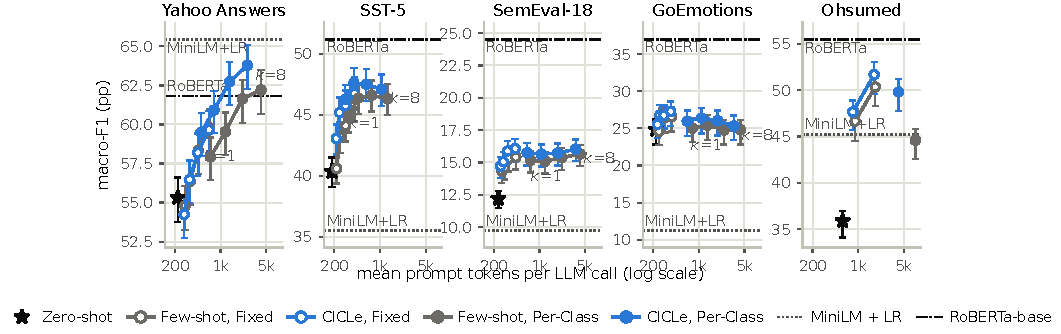
\includegraphics[width=\textwidth]{figures/f1_vs_tokens.pdf}
  \caption{Macro-F1 against mean prompt tokens per LLM call (log scale), one panel per dataset. Every point is one (method, retrieval variant, $k$) at the reference setting, averaged over six models and three seeds, with $k$ increasing along each line. Hollow markers: Fixed retrieval. Filled: Per-Class. Grey: few-shot. Blue: CICLe. Star: zero-shot. Dotted and dash-dot lines: MiniLM with logistic regression and fine-tuned RoBERTa-base (three-seed means). Error bars are 95\% bootstrap intervals of the 18-run mean over test instances, not the spread over hyperparameters. Ohsumed Per-Class is $k = 1$ only.}
  \label{fig:tokens}
\end{figure*}


\subsection{How You Narrow Matters}
\label{sec:res-narrowing}
% CLAIM: At equal mean set size CP = top-k = mass on balanced data; under a long-tailed labelled pool the
% alternatives lose coverage on rare classes and 4-11 macro-F1 points. Imbalance does NOT widen the
% CICLe-vs-few-shot gap (explicit retraction of the pilot's claim). Coverage bounds the damage (fixes vs breaks).
% Appendix figure (text width): fig_app_narrowing_extra.pdf, the panels of the narrowing analysis not shown in Figure 2.
\begin{figure*}[t]
  \centering
  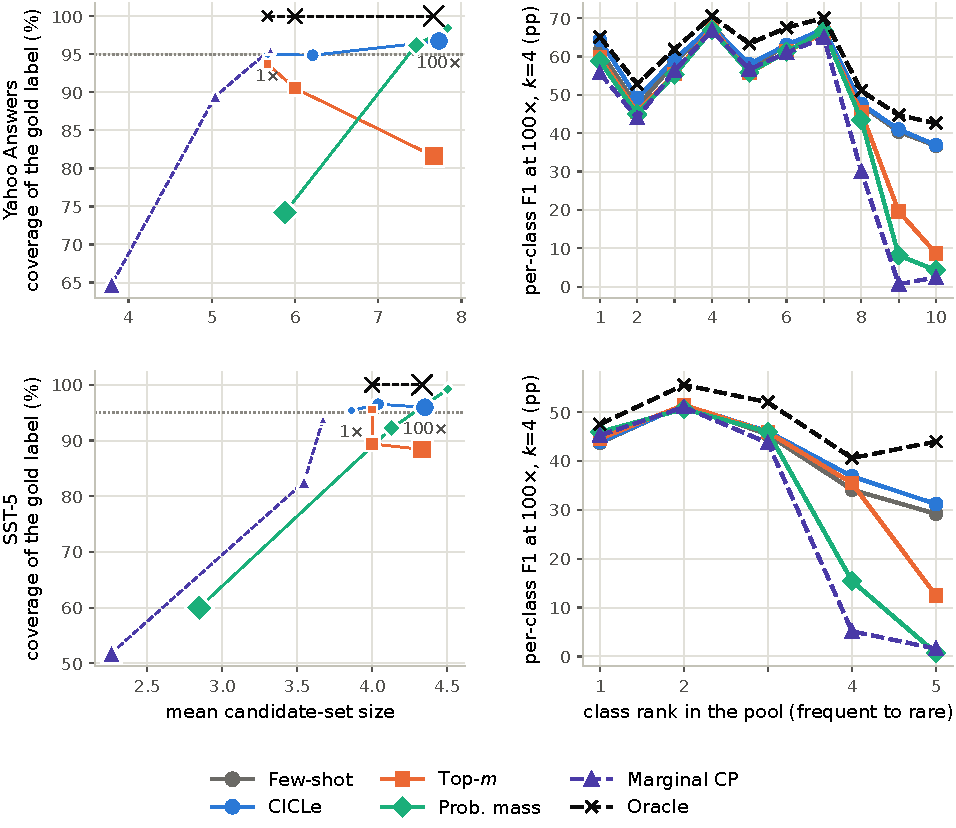
\includegraphics[width=\textwidth]{figures/fig_app_narrowing_extra.pdf}
  \caption{Further panels of the narrowing analysis (Per-Class retrieval, rows Yahoo Answers and SST-5). Left: coverage of the gold label against mean candidate-set size for every rule at 1, 10 and 100 times imbalance (marker size grows with imbalance), mean over three seeds, with the $1 - \alpha$ target dotted. Right: per-class F1 at 100 times imbalance and $k = 4$ by class-frequency rank in the pool, mean over six models and three seeds.}
  \label{fig:imbalance}
\end{figure*}


\subsection{Uninformative Label Names}
\label{sec:res-relabel}
% CLAIM: With every label renamed to a nonsense word, CICLe's margin over few-shot is the largest measured
% (+6.5 Fixed / +5.6 PC on Yahoo; +0.7 / +1.0 on GoEmotions, 36 pairs).
% Table 3 (column width): original vs renamed labels. Spec: figures_and_tables.md. PLACEHOLDER.
\begin{table}[t]
  \centering
  \small
  % TODO: Dataset | Labels | k | Few-shot Fixed | CICLe Fixed | Few-shot PC | CICLe PC; Yahoo and GoEmotions, k in {1,4}; final row paired delta on renamed labels (36 pairs).
  \begin{tabular}{llrrrrr}
    \toprule
    Dataset & Labels & $k$ & FS-F & CICLe-F & FS-PC & CICLe-PC \\
    \midrule
    \multicolumn{7}{c}{\emph{placeholder}} \\
    \bottomrule
  \end{tabular}
  \caption{Macro-F1 with the original label names and with every class renamed to a nonsense word (same mapping for all seeds). The base classifier is unaffected, so the whole effect is on the LLM's use of the candidate list. FS: few-shot. F: Fixed. PC: Per-Class.}
  \label{tab:relabel}
\end{table}


\subsection{When the LLM Pipeline Is Worth It}
\label{sec:res-baselines}
% CLAIM: With 1,600 balanced labels fine-tuned RoBERTa-base beats every pipeline on 4 of 5 datasets and the
% base classifier alone wins on Yahoo; at 100x imbalance the order flips. [PENDING pool size.] Decision rule.
% Table 4 (appendix, full width). Body generated by make_figures.py (tab4).
\begin{table*}[t]
  \centering
  \scriptsize
  \setlength{\tabcolsep}{3pt}
  % Table 4. Macro-F1; supervised rows mean over 3 seeds, LLM rows over 6 models x 3 seeds. Zero-shot does not depend on the pool (1x column only). F = Fixed retrieval (Ohsumed has no Per-Class runs). Bold = best per column.
\begin{tabular}{lccccccccc}
\toprule
 & Yahoo Answers 1$\times$ & Yahoo Answers 10$\times$ & Yahoo Answers 100$\times$ & SST-5 1$\times$ & SST-5 10$\times$ & SST-5 100$\times$ & SemEval-18 & GoEmotions & Ohsumed \\
\midrule
MiniLM + LR & \textbf{65.4} & 50.4 & 31.4 & 35.5 & 20.5 & 12.6 & 9.7 & 11.2 & 45.2 \\
RoBERTa-base, fine-tuned & 61.8 & 58.7 & 41.2 & \textbf{51.2} & 44.5 & 31.9 & \textbf{24.5} & \textbf{37.0} & 55.4 \\
RoBERTa-large, fine-tuned & 64.6 & \textbf{61.6} & 44.9 & 39.9 & 35.8 & 32.2 & 23.0 & 27.3 & \textbf{66.1} \\
Zero-shot & 55.3 & -- & -- & 40.3 & -- & -- & 12.2 & 24.9 & 35.9 \\
Few-shot PC, $k$=4 & 61.6 & 59.4 & 54.6 & 46.6 & 44.6 & 40.8 & 15.4 & 24.8 & 50.4\textsuperscript{F} \\
CICLe PC, $k$=4 & 62.7 & 60.3 & 55.4 & 47.5 & \textbf{46.5} & 41.9 & 15.7 & 26.0 & 51.7\textsuperscript{F} \\
Best LLM pipeline & 63.8 {\scriptsize CICLe PC $k$=8} & 60.3 {\scriptsize CICLe PC $k$=4} & \textbf{56.0} {\scriptsize CICLe PC $k$=1} & 47.6 {\scriptsize CICLe PC $k$=2} & \textbf{46.5} {\scriptsize CICLe PC $k$=4} & \textbf{43.4} {\scriptsize CICLe PC $k$=1} & 16.1 {\scriptsize CICLe F $k$=8} & 27.3 {\scriptsize CICLe F $k$=8} & 53.1 {\scriptsize CICLe F $k$=8} \\
\bottomrule
\end{tabular}

  \caption{Supervised baselines against LLM pipelines, macro-F1. Supervised rows are means over three seeds, LLM rows over six models and three seeds. The fixed configuration is Per-Class retrieval at $k = 4$ (Ohsumed: Fixed, marked F). The best pipeline is the best (method, variant, $k$) mean per column and is selected on the test set. Zero-shot prompting does not depend on the pool. The test sample is identical at every imbalance level. Bold marks the best value per column.}
  \label{tab:baselines}
\end{table*}


\subsection{Choosing $\alpha$, and Robustness Across Models}
\label{sec:res-alpha}
% CLAIM: A looser alpha pays where the classifier is strong (Yahoo) or sets are otherwise huge (GoEmotions),
% is flat on SST; embedding matters more than classifier; no model is hurt by PC CICLe; 12B and 32B models
% also gain (Appendix F); a 3B model with CICLe PC matches 32B zero-shot on the same seed.
% Figure 3 (column width, two stacked panels): choosing alpha. Spec: figures_and_tables.md. PLACEHOLDER.
% Candidate for the appendix if the page budget bites (presentation_plan.md, resolution (a)).
\begin{figure}[t]
  \centering
  % 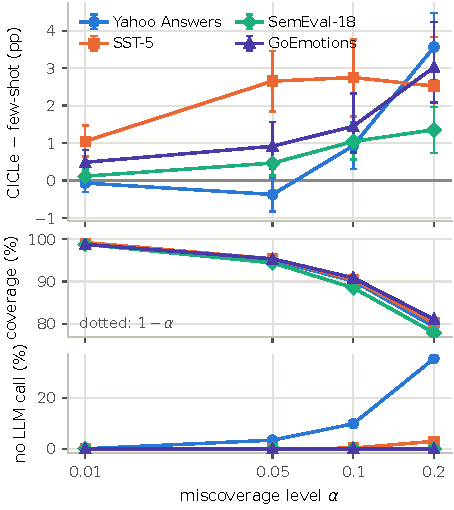
\includegraphics[width=\columnwidth]{figures/alpha.pdf}
  \fbox{\parbox{0.95\columnwidth}{\centering\vspace{3em}\emph{Figure 3 placeholder: $\Delta$ vs.\ few-shot and LLM-skip rate against $\alpha$}\vspace{3em}}}
  \caption{Effect of the miscoverage level $\alpha$. Top: paired difference CICLe minus few-shot, one line per dataset (Llama-3.1-8B and Llama-3.2-3B, 24 cells). Bottom: share of test instances answered by the base classifier alone. Annotations give the empirical coverage at each $\alpha$.}
  \label{fig:alpha}
\end{figure}

